\documentclass[tikz, border=10pt]{standalone}
\usetikzlibrary{automata, positioning, arrows, calc, shapes.geometric}

\begin{document}

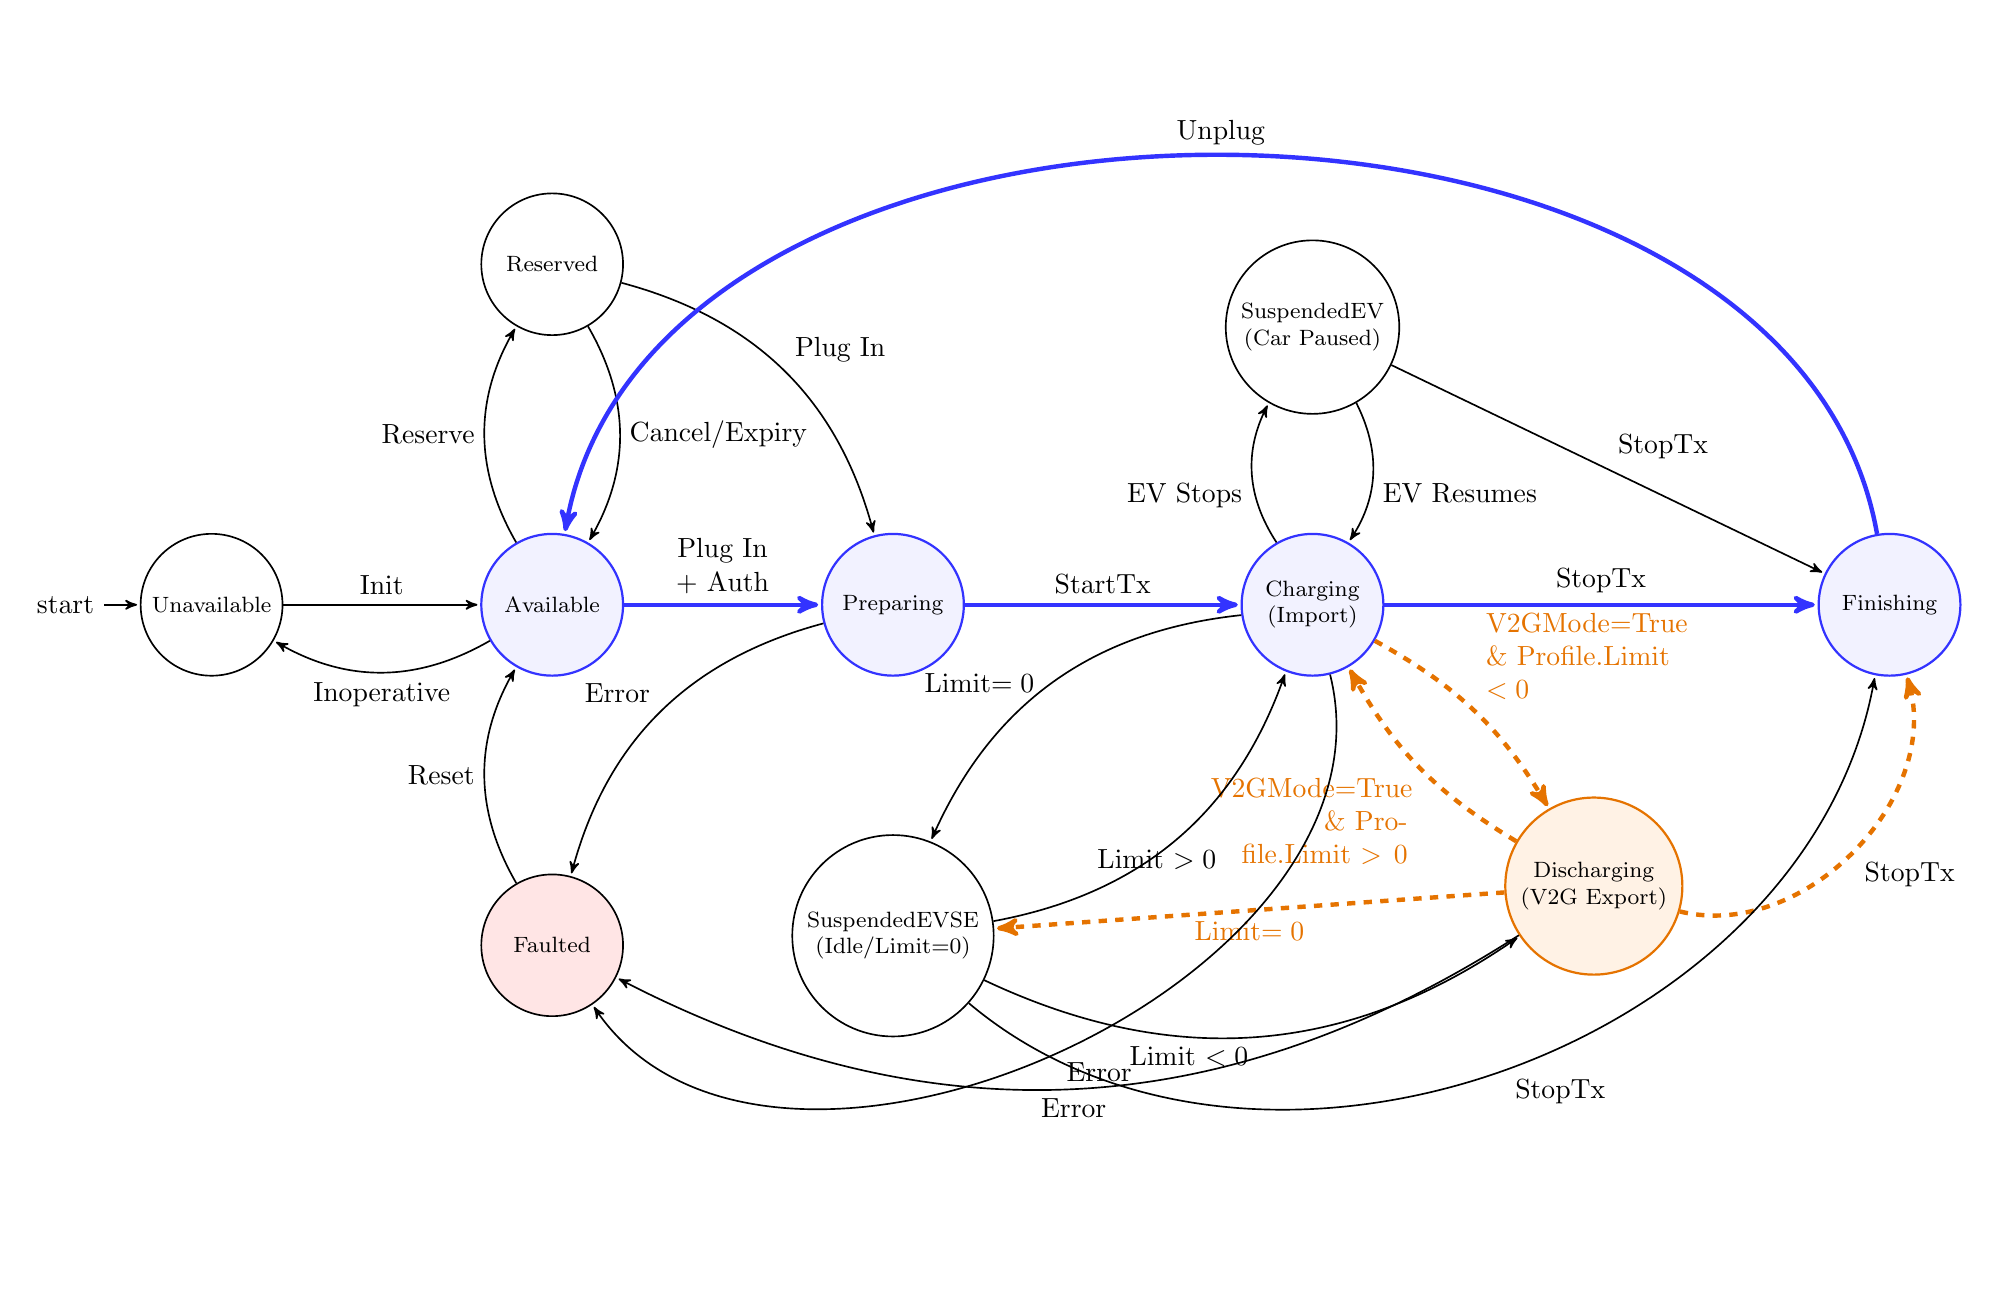
\begin{tikzpicture}[>=stealth', shorten >=1pt, auto, node distance=2.5cm, semithick]
  % Styles
  \tikzstyle{every state}=[fill=white, draw=black, text=black, font=\footnotesize, minimum size=1.8cm, align=center]
  \tikzstyle{mainloop}=[draw=blue!80, ultra thick]
  \tikzstyle{v2gloop}=[draw=orange!90!black, ultra thick, dashed]
  \tikzset{mainnode/.style={fill=blue!5, draw=blue!80, thick}}
  \tikzset{v2gnode/.style={fill=orange!10, draw=orange!90!black, thick}}

  % --- Nodes ---
  \node[initial, state] (Unavailable) {Unavailable};
  \node[state, mainnode] (Available) [right=of Unavailable] {Available};
  \node[state] (Reserved) [above=of Available] {Reserved};
  \node[state, mainnode] (Preparing) [right=of Available] {Preparing};
  
  % Central Operation Block
  \node[state, mainnode] (Charging) [right=3.5cm of Preparing] {Charging\\(Import)};
  \node[state, v2gnode] (Discharging) [below right=3cm of Charging] {Discharging\\(V2G Export)};
  
  % Suspended States
  \node[state] (SuspendedEV) [above=1.5cm of Charging] {SuspendedEV\\(Car Paused)};
  \node[state] (SuspendedEVSE) [below=2cm of Preparing] {SuspendedEVSE\\(Idle/Limit=0)};
  
  % End State
  \node[state, mainnode] (Finishing) [right=5.5cm of Charging] {Finishing};
  
  % Fault State
  \node[state, fill=red!10] (Faulted) [below=of Available] {Faulted};

  % --- Transitions ---

  % 1. Setup & Init
  \path[->] 
    (Unavailable) edge [] node {Init} (Available)
    (Available) edge [bend left] node {Inoperative} (Unavailable)
    (Available) edge [bend left] node {Reserve} (Reserved)
    (Reserved) edge [bend left] node {Cancel/Expiry} (Available)
    (Available) edge [mainloop] node [text width=2cm, align=center] {Plug In\\+ Auth} (Preparing)
    (Reserved) edge [bend left] node {Plug In} (Preparing);

  % 2. Preparing to Operations
  \path[->]
    (Preparing) edge [mainloop] node {StartTx} (Charging)
    (Preparing) edge [bend right] node [swap] {Error} (Faulted);

  % 3. Charging Loops & V2G Logic (CORE MEA REQUIREMENT)
  \path[->]
    % Charge -> V2G
    (Charging) edge [v2gloop, bend left=15] node [text width=2.5cm, align=left, color=orange!90!black] 
    {V2GMode=True\\\& Profile.Limit $< 0$} (Discharging)
    
    % V2G -> Charge
    (Discharging) edge [v2gloop, bend left=15] node [text width=2.5cm, align=right, color=orange!90!black] 
    {V2GMode=True\\\& Profile.Limit $> 0$} (Charging)
    
    % Charge -> Idle (Limit 0)
    (Charging) edge [bend right] node [text width=1.5cm, left] {Limit$=0$} (SuspendedEVSE)
    
    % V2G -> Idle (Limit 0)
    (Discharging) edge [v2gloop] node [below, color=orange!90!black] {Limit$=0$} (SuspendedEVSE)
    
    % Idle -> Charge/V2G
    (SuspendedEVSE) edge [bend right] node [below, text width=2cm] {Limit $> 0$} (Charging)
    (SuspendedEVSE) edge [bend right] node [below left] {Limit $< 0$} (Discharging);

  % 4. Suspended EV (Car Control)
  \path[->]
    (Charging) edge [bend left] node {EV Stops} (SuspendedEV)
    (SuspendedEV) edge [bend left] node {EV Resumes} (Charging);

  % 5. Finishing & Stops
  \path[->]
    (Charging) edge [mainloop] node {StopTx} (Finishing)
    (Discharging) edge [v2gloop, bend right=60] node [swap] {StopTx} (Finishing)
    (SuspendedEV) edge [] node {StopTx} (Finishing)
    (SuspendedEVSE) edge [bend right=60] node [swap] {StopTx} (Finishing)
    
    (Finishing) edge [bend right=80, mainloop] node [above] {Unplug} (Available);

  % 6. Faults
  \path[->]
    (Charging) edge [bend left=80] node {Error} (Faulted)
    (Discharging) edge [bend left] node {Error} (Faulted)
    (Faulted) edge [bend left] node {Reset} (Available);

\end{tikzpicture}

\end{document}